\documentclass[a4paper]{article}
\usepackage[utf8]{inputenc}
\usepackage[spanish, es-tabla, es-noshorthands]{babel}
\usepackage[table,xcdraw]{xcolor}
\usepackage[a4paper, footnotesep = 1cm, width=20cm, top=2.5cm, height=25cm, textwidth=18cm, textheight=25cm]{geometry}
%\geometry{showframe}

\usepackage{tikz}
\usepackage{amsmath}
\usepackage{amsfonts}
\usepackage{amssymb}
\usepackage{float}
\usepackage{graphicx}
\usepackage{caption}
\usepackage{subcaption}
\usepackage{multicol}
\usepackage{multirow}
\setlength{\doublerulesep}{\arrayrulewidth}
\usepackage{booktabs}

\usepackage{hyperref}
\hypersetup{
    colorlinks=true,
    linkcolor=blue,
    filecolor=magenta,      
    urlcolor=blue,
    citecolor=blue,    
}

\newcommand{\quotes}[1]{``#1''}
\usepackage{array}
\newcolumntype{C}[1]{>{\centering\let\newline\\\arraybackslash\hspace{0pt}}m{#1}}
\usepackage[american]{circuitikz}
\usetikzlibrary{calc}
\usepackage{fancyhdr}
\usepackage{units} 

\graphicspath{{../Calculos-Potencia/}{../Caracteristicas/}{../Consideraciones/}{../Gain-Stage/}{../Input-Stage/}{../Output-Stage/}{../Simulaciones/}{../Alimentacion/}{../Conclusiones/}}

\pagestyle{fancy}
\fancyhf{}
\lhead{22.12 Electrónica II}
\rhead{Mechoulam, Lambertucci, Rodriguez, Londero, Scala}
\rfoot{Página \thepage}

\begin{document}
El circuito final es el que se presenta a continuación:
 \begin{figure}[H]
\centering
	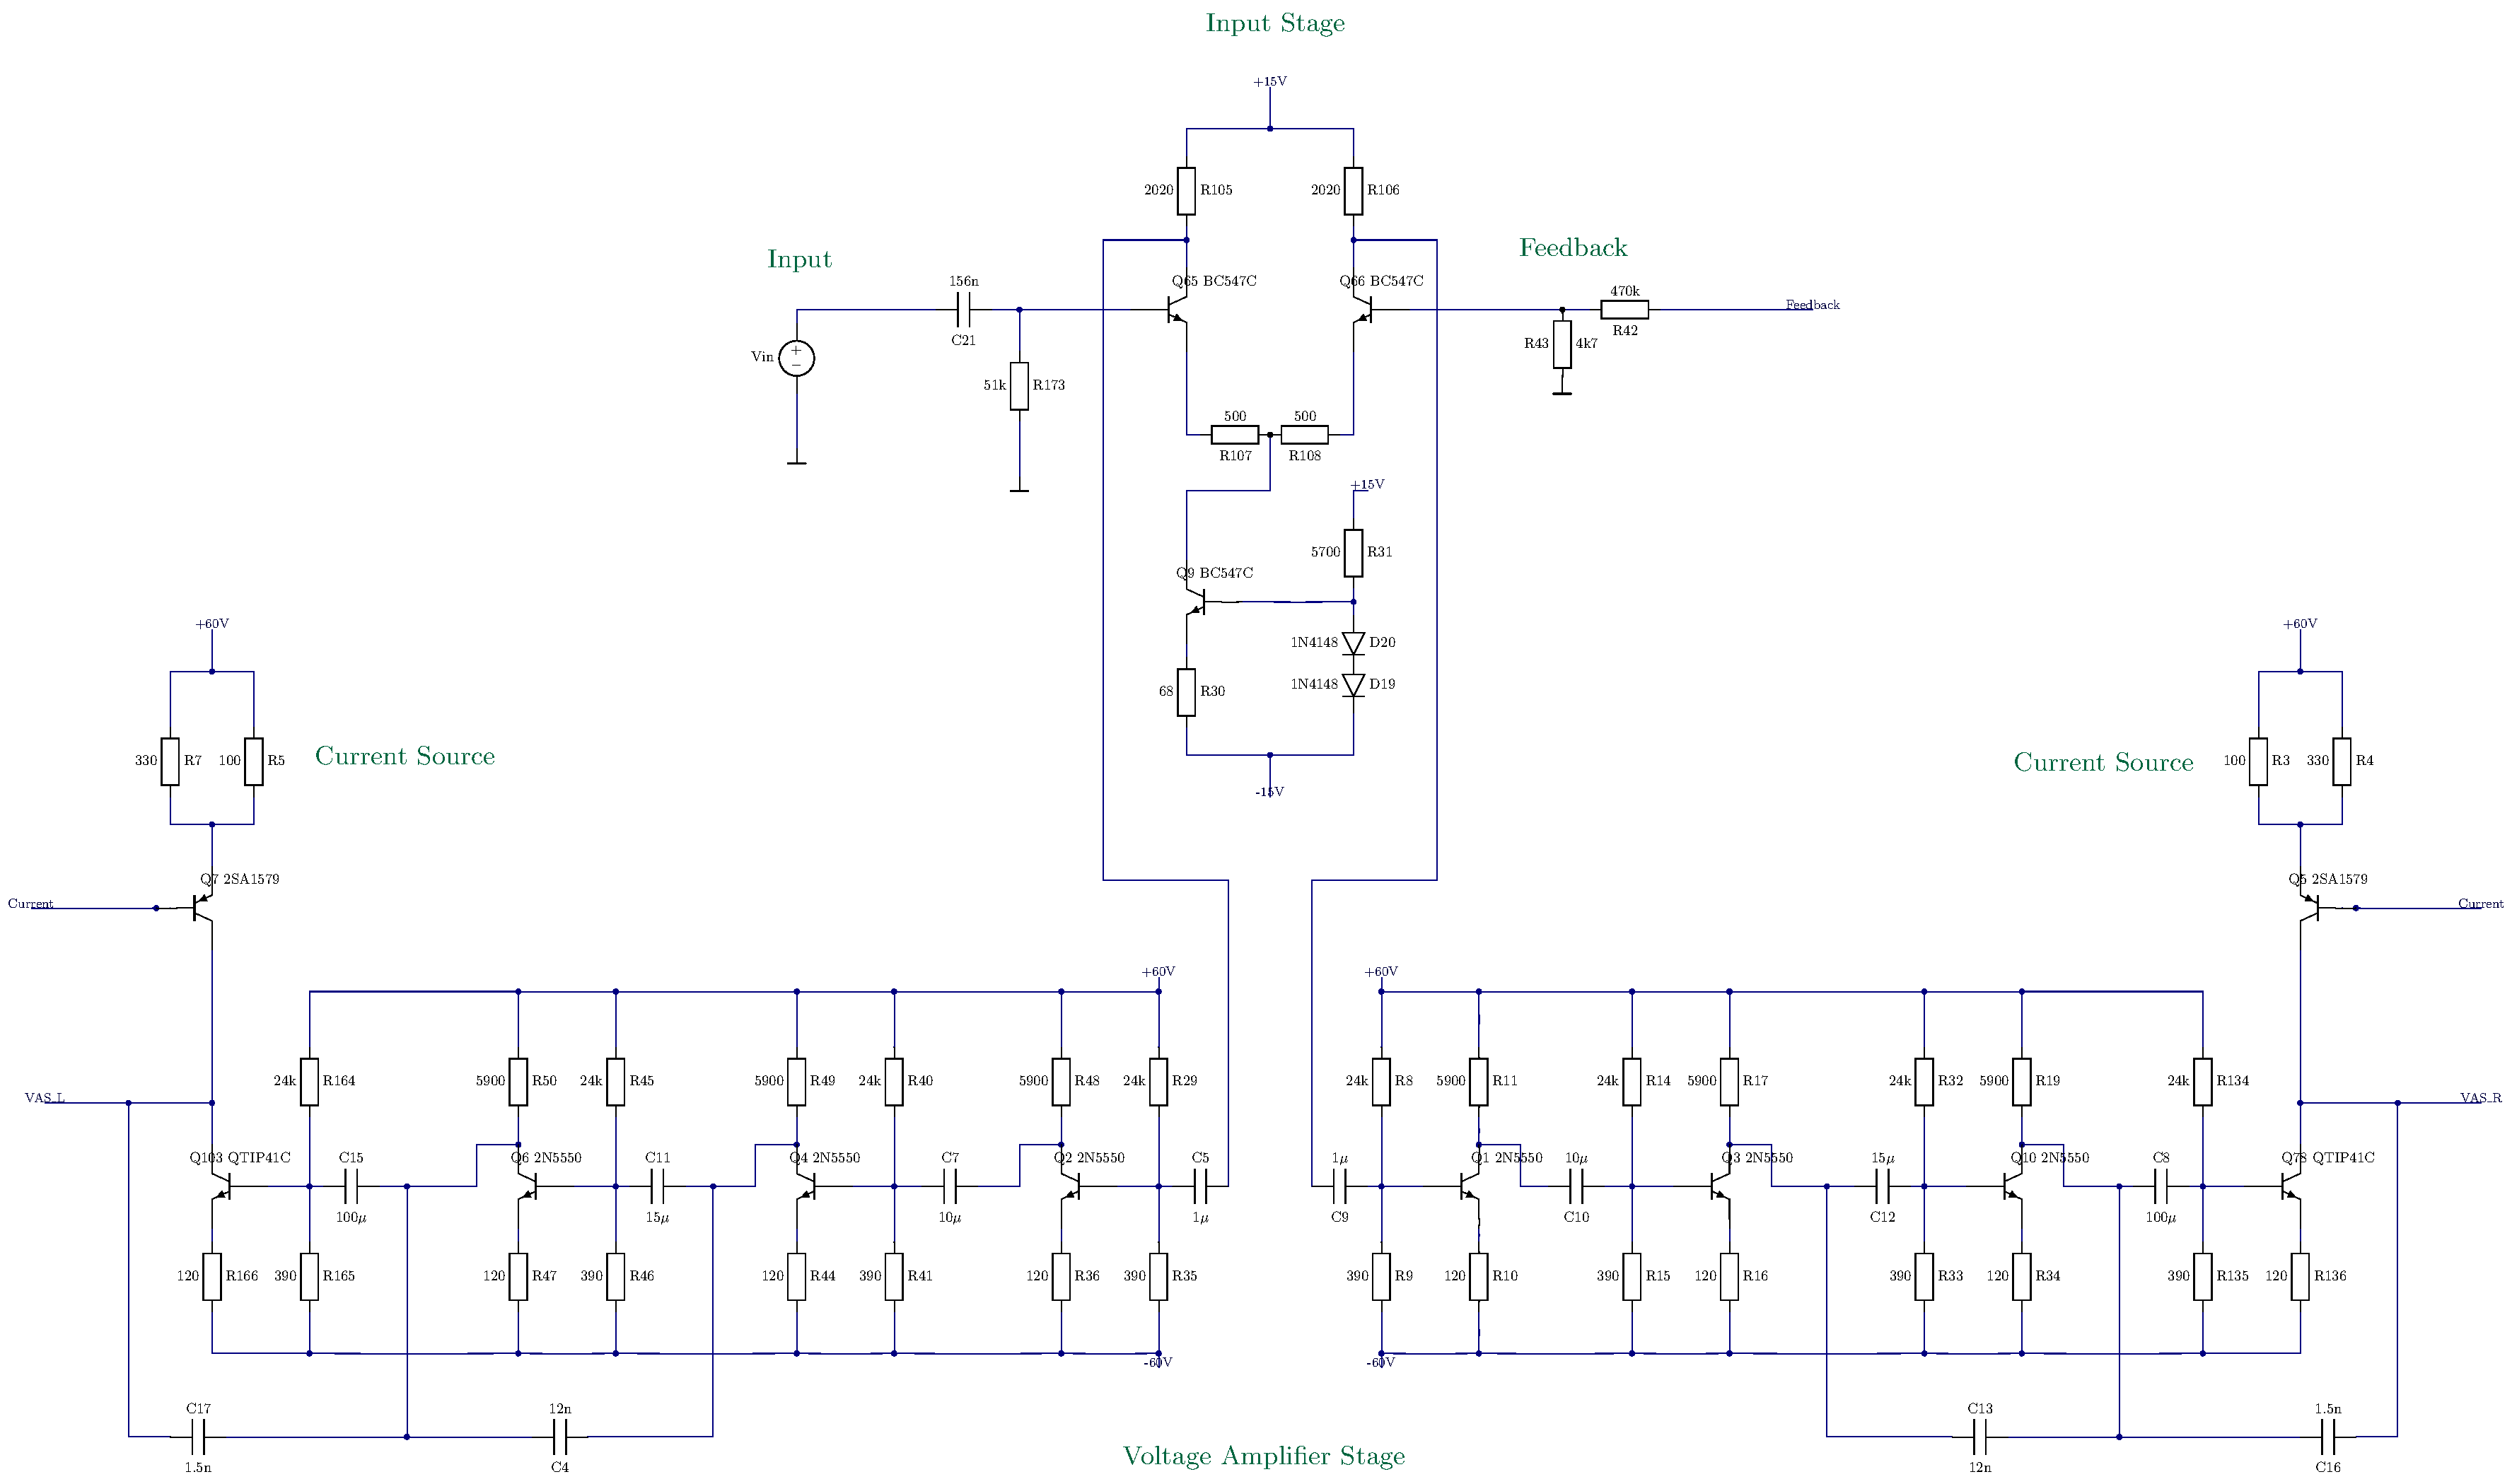
\includegraphics[width=\textwidth]{ImagenesCaracteristicas/TEX1.pdf}
	\caption{Etapas de entrada y amplificación}
	\label{fig:circ}
\end{figure}
 \begin{figure}[H]
\centering
	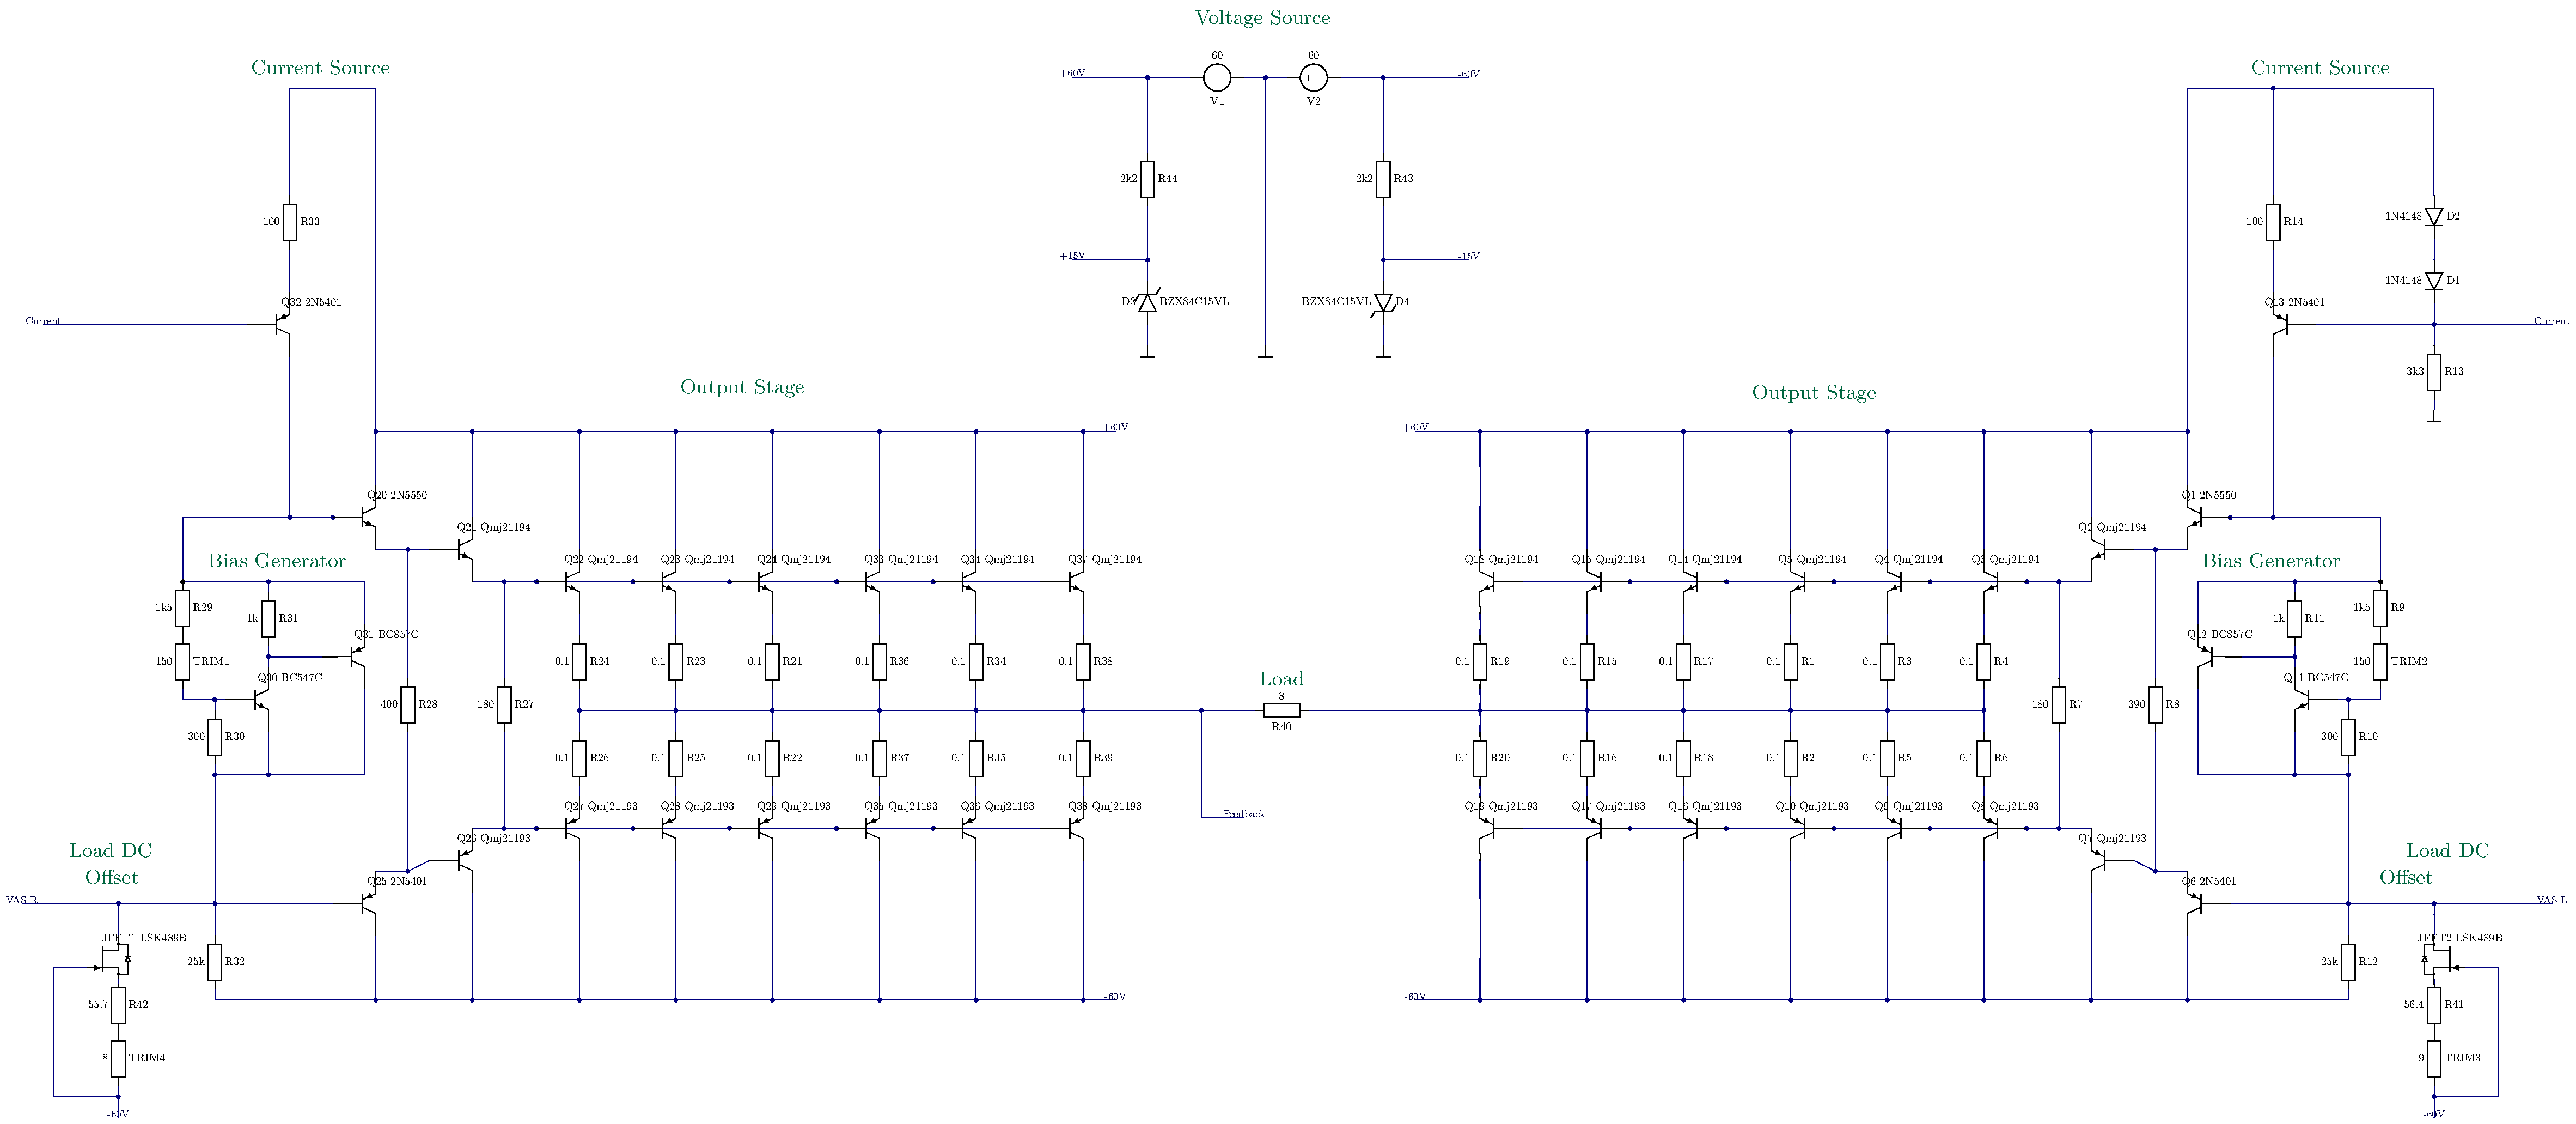
\includegraphics[width=\textwidth]{ImagenesCaracteristicas/TEX2.pdf}
	\caption{Etapas de salida y carga}
	\label{fig:circ}
\end{figure}

Ahora se mencionan algunas características notables del circuito:
\begin{itemize}
\item Cuentas con una potencia máxima de 1kW
\item Configuración de puente H  para la carga.
\item Rendimiento del amplificador balanceado del 74.5$\%$
\item En los extremos de la banda audible, correspondientes a la respuesta en frecuencia es de -3dB respecto a la banda de paso.

\item El circuito se mantiene estable frente a ruido de distinta naturaleza y mantiene una salida senoidal.

\item Cuenta con una impedancia de entrada de 50k$\Omega$ en toda la banda de paso.
\item La impedancia de salida es pequeña, del orden de las decenas de m$\Omega$, aunque el valor óptimo para esta es de 8$\Omega$ para que haya máxima transferencia de potencia.


\item Cuenta con una distorsión armónica del $\%$
\item Se obtiene una tensión de 180$V_{pp}$ con una fuente de  alimentacion de $\pm 60V$
\item El circuito cuenta con la cualidad de de ajustar el nivel de continua sobre la carga.
\item Permite calibrar el nivel de continua en reposo sobre los transistores de salida.
\item Implementación con una única fuente partida.



\end{itemize}

\end{document}